\documentclass{article}
\usepackage{graphicx} % Required for inserting fig

\usepackage{subfig}
\usepackage[hidelinks]{hyperref}
\usepackage{rotating}
\usepackage{comment}

\setlength{\parskip}{16pt}

\title{Final project assignment:\@ Simulation of a base scenario }

\author{Jef Jacobs \\ Toon Eeraerts \\ Wout Deleu}
\date{Semester 2}

\begin{document}
\setlength{\parindent}{0pt} \maketitle \tableofcontents \newpage %geen indent bij nieuwe paragraaf

\maketitle
\newpage

\section{Introduction}
In this report, the final assignment of the 'Yard Storage Assignment Problem'
is discussed. The focus of this assignment consisted of designing a simulation
to visualize a port complex and analyse the storage occupancy in the yard.
Python is the primary technology used for this dynamic simulation, with global
variables and booleans controlling its flow. The simulation is based on
discrete data but is in itself an online simulation, using a stream of newly
generated data, based on the discrete data, as input.

The goal is to simulate container groups arriving and departing from the yard,
where they are typically stored together without being split up. This
simulation aims to simulate the storage in the yard resulting from the inflow
and outflow of containers. Three additional scenarios have been implemented to
provide new insights into how the yard operates. Additionally, a visualization
feature has been implemented. This visualization was one of the primary goals
for this semester and serves as the finishing touch for this course. It brings
the entire project together, making all the realizations visible, and provides
genuine insights into the movements of the various elements within the yard.

\begin{comment} To summarize, the focus of the first lab was on analyzing the existing data
samples. The intention was to be able to sample them throughout the project to
approximate reality. The objective of the second assignment was to set up a
base scenario for simulation and obtain initial results. The samples obtained
from previous sessions were converted into usable distributions and used to
generate parameters for the container arrival and departure schedule. With a
basic simulation scenario in place, the initial results could be examined. It
is important to note that some minor errors occurred during the development and
design of the sample functions. These errors stemmed from a misinterpretation
of the graphs from the initial reports, resulting in a significant
underestimation of the number of generated containers. This issue was also
mentioned in the second report. However, while designing the final simulation,
the mistake resurfaced but was promptly identified and resolved, no longer
posing a problem.
\end{comment}

\section{Probability distributions}
The simulation makes use of probability distributions derived from real yard
data provided by Ir. E. Thanos. Each distribution is carefully designed to have
the same average results as the input data. The simulation involves generating
samples of container groups, each having distinct characteristics determined by
these distributions.

\subsection{Inter arrival time}
The sampling frequency of container groups is a critical parameter in the
simulation. In the original input data, container groups frequently arrived at
the same time on the same vessel, leading to a high occurrence of zero
inter-arrival times, shown in Figure~\ref{fig:inter-arrival times real}.
Consequently, the average inter-arrival time has a very low value of 0.092
hours or 5 minutes and 30 seconds.

To ensure a representative distribution, this average value had to be present
in our sample distribution. To represent the steepness of the graph, an
exponential function was used, resulting in the distribution shown in
Figure~\ref{fig:inter-arrival times sample}.

\begin{figure}[!tbp]
    \centering
    \subfloat[Real distribution]{
        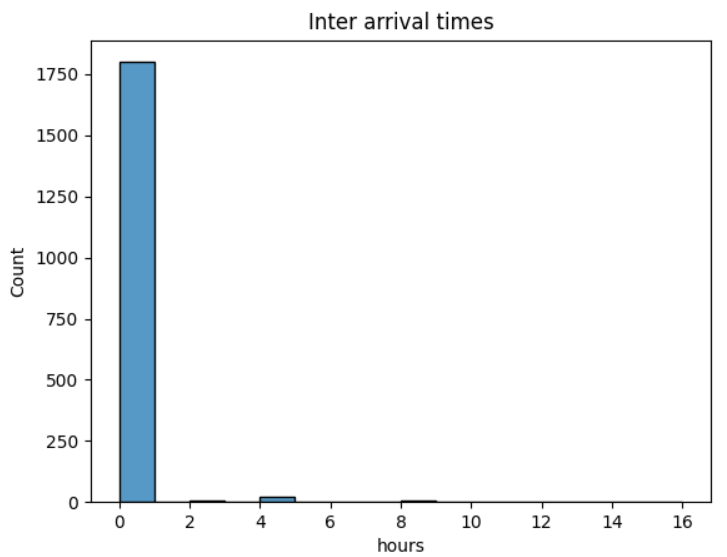
\includegraphics[width=0.48\textwidth]{fig/input data - inter-arrival times.png}\label{fig:inter-arrival times real}}
    \hfill
    \subfloat[Sample distribution]{
        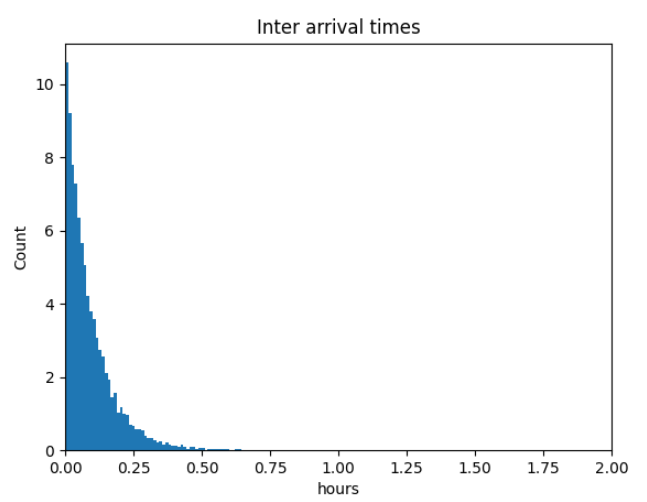
\includegraphics[width=0.48\textwidth]{fig/sample inter-arrival times.png}\label{fig:inter-arrival times sample}}
    \caption{Inter-arrival times}
\end{figure}

\subsection{Container group size}
The container group sizes in the input data indicate significant variance,
ranging from single-container groups to groups with over 2000 containers. This
strong variance caused a difficult decision in determining an appropriate
distribution. In the end, a Weibull distribution was chosen to achieve a steep
descent at the lower end while simultaneously allowing for the possibility of
larger group sizes. The average size of container groups in the input data, as
shown in Figure~\ref{fig:cg_sizes_real}, is 32 containers. The Weibull
distribution used for this sample generation is shown in
Figure~\ref{fig:cg_sizes_sample}.

Based on the previous average outcome, we can calculate the weekly generation
of containers. This number corresponds to the quantity of containers being
transported each week. The result is nearly identical to the number of
containers from the input data, thereby validating the average values of the
preceding distributions.

\begin{equation}
    Generated\_containers = \frac{Total\_time}{inter\_arrival\_time} \cdot Average\_container\_group\_size \end{equation}
\begin{equation} = \frac{168}{0.091} \cdot 32 \end{equation}
\begin{equation} \approx 59000 \end{equation}

\begin{figure}[!tbp]
    \centering
    \subfloat[Real distribution]{
        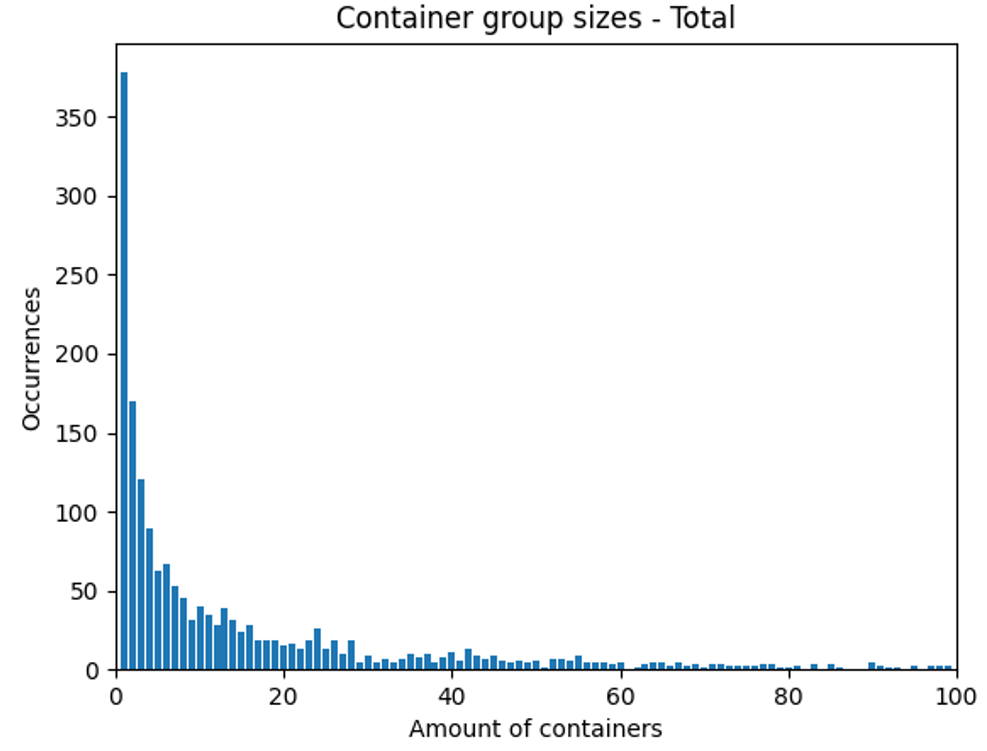
\includegraphics[width=0.48\textwidth]{fig/input data - cg sizes.png}
        \label{fig:cg_sizes_real}}
    \hfill
    \subfloat[Sample distribution]{
        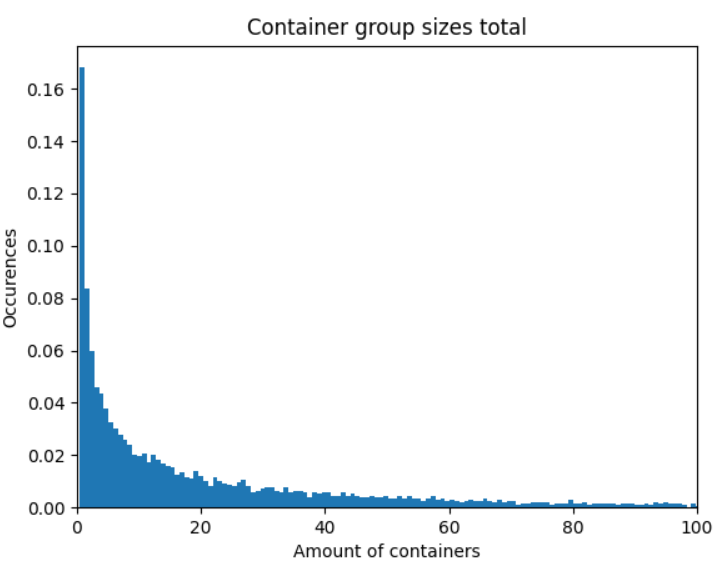
\includegraphics[width=0.48\textwidth]{fig/sample cg sizes.png}
        \label{fig:cg_sizes_sample}}
    \caption{Container group sizes}
\end{figure}

\subsection{Service time}
The service time of each container group represents how long they stay in the
yard before departing. The input data revealed a uniform distribution ranging
from zero to 166 hours, shown in Figure~\ref{fig: service sample distribution}.
However, it is important to note that this distribution only represents the
container groups falling under transshipment. The other kind of container
groups (export and import) always have a service time of 48 hours.

Although generating consistent container groups with a 48-hour service time
would be interesting, the distribution was simplified due to the larger number
of transshipment container groups compared to the other types. The resulting
distribution is a unfiorm distribution between zero and 166 hours.

\begin{figure}
    \centering
    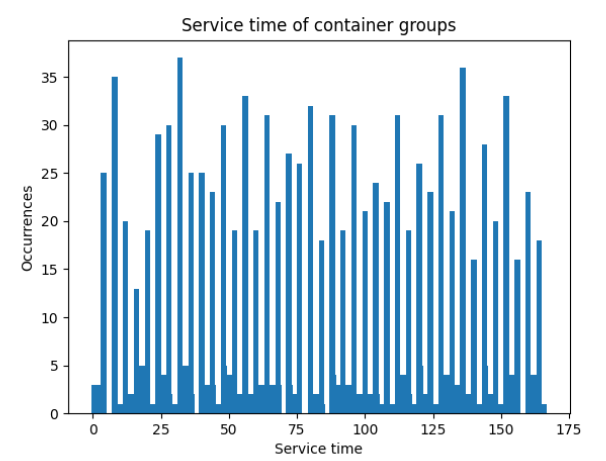
\includegraphics[width=0.5\textwidth]{fig/service time analysis.png}
    \caption{Service time sample distribution}\label{fig: service sample distribution}
\end{figure}

\subsection{Container type}
Each container group can be of normal or reefer type. This distribution was
based upon the input analysis of Nick De Bruyckere, Enrique Miron and Dries Van
de Velde represented in Figure~\ref{fig:container type analysis}. Normal
containers and reefer container occur respectively 69\% and 31\% of the times.

\begin{figure}
    \centering
    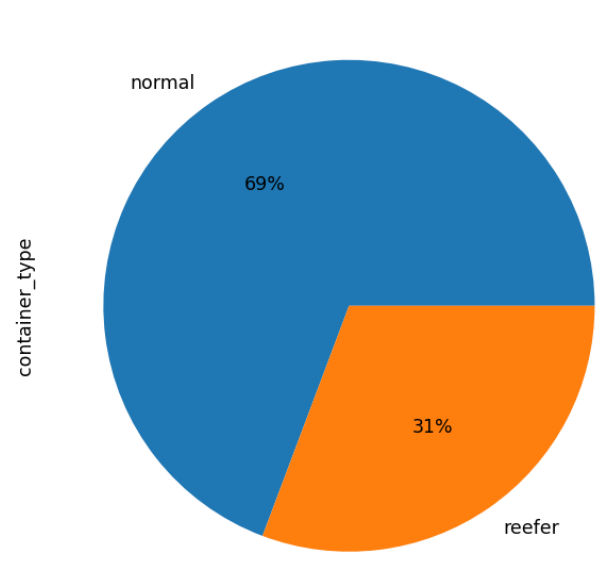
\includegraphics[width=0.5\textwidth]{fig/container_type.png}
    \caption{Container type analysis}\label{fig:container type analysis}
\end{figure}

\subsection{Arrival and departure points}
The arrival and departure positions of vessels and trucks are chosen randomly
from the available locations. The selection of either a vessel location or a
truck location depends on the flow type, which is disccused in the next
chapter.

\subsection{Flow type}
Each container group can be categorized as either export or import. In the
input data, all groups that were categorized as transshipment are now
categorized as export. The distribution of these flow types is based on the
proportion of containers in the input data belonging to each category,
resulting in 81\% export and 19\% import.

For the container groups classified as export, further division was necessary
to determine their berthing locations and potential truck locations. This is
because transshipment's would go from vessel to vessel, while true exports from
truck to vessel. This distribution resulted in 69\% transshipment's and 31\%
true export.

\section{Algorithm}
In this section, the flow, architecture and the design of the code are
discussed. Since this code was developed in multiple steps, each with its own
objectives, the program exhibits a highly modular structure. This modularity
proved to be particularly advantageous for potential code reuse.

\subsection{Amount of simulations}
One crucial parameter to determine is the number of simulations required to
obtain significant results. This can be calculated using the following formula: \[S = \sqrt{\frac{\sum_{i = 1}^{n}(X_i-\overline{X})^2}{n
            -1}}\] \[\frac{S}{\sqrt{k}} < d\]

The most important parameter is the travel distance, denoted as X. To ensure
the reliability of the outcomes, we use the sample variance, denoted as S. The
number of simulations performed is represented by k. Additionally, we define an
accepted standard deviation, denoted as d. This threshold can be chosen based
on the desired level of accuracy or confidence in the results.

In our case, X represents either the average or total travel distance obtained
from running the simulation. The calculation process involves repeatedly
running the simulation and collecting X values. As the number of simulations
increases, the sample variance based on these k values is continuously
evaluated. Once the sample variance falls within an acceptable range determined
by the chosen standard deviation d, the calculation process is stopped, and the
value of k is selected as the number of simulations required to achieve the
desired level of accuracy.

For the total distance the accepted deviation is 1000. If we look at the
magnitude of the total travel distance, we see it surpasses a million. A
deviation of a thousands seems in that case reasonable. The total distance
travelled is a much larger value than the average, because of this the accepted
deviation is larger. From this information we can conclude that at least 120
simulations must be done to get consistent results.

\begin{figure}[h]
    \centering
    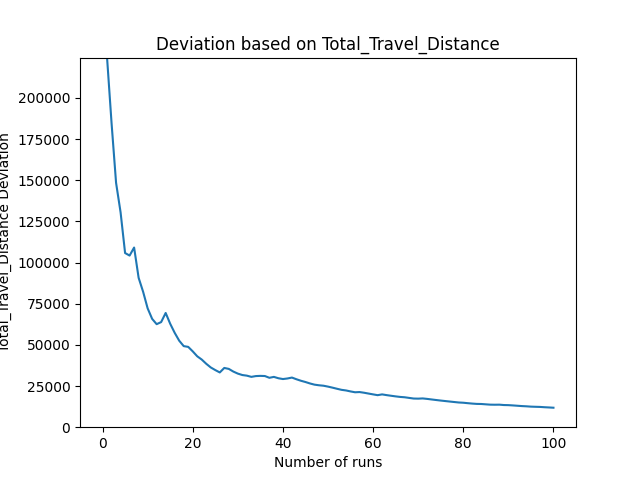
\includegraphics[width=0.7\textwidth]{fig/calcruns.png}
    \caption{Deviation based on total travel distance}\label{fig:amount_of_runs}
\end{figure}

\subsection{Flow}
Due to the requirement of testing multiple scenarios in the simulation,
designing and structuring the program to allow for flexible flow manipulation
without significant internal changes posed a challenge. To address this, the
program utilizes booleans to map out different paths within the simulation.
These booleans serve as input parameters and can be configured to define
predefined scenarios. To ensure consistency and prevent unintended
configurations, checks are implemented to throw exceptions if the booleans are
set in an invalid combination. In the current implementation, four booleans
were utilized:
\begin{enumerate}
    \item ARRIVAL BASED
    \item DEPARTURE BASED
    \item CLOSEST
    \item LOWEST OCCUPANCY
    \item MIXED RULE
    \item SPLIT UP
\end{enumerate}

\subsection{Core}
The program operates on an event-based model, where the simulation timer
progresses from one event to another. To achieve this, two lists are maintained
to hold the events: one for container arrivals at the yard and another for
container departures from the yard. Whenever a container is generated, a new
arrival event is scheduled based on the interarrival time sampling function.
Upon arrival, the container is checked to see if there is available space in
the yard for storage. If there is, a yard block is selected based on the
defined scenario to store the container. However, if there is no available
space, the container is rejected.

In events where containers depart, the respective container is removed from the
yard. For each event that occurs, all relevant statistics are updated. This
process continues until the simulation time is reached, completing the
simulation.

\subsection{Visualization}
The visualization component of the simulation is implemented using Tkinter, a
Python library widely used for creating graphical user interfaces (GUIs).
Tkinter is based on the Tk GUI toolkit, hence its name "Tkinter." One of the
key advantages of Tkinter is its inclusion in the standard Python distribution,
eliminating the need for additional library installations. This accessibility
makes it beginner-friendly and convenient for developing cross-platform
applications.

In summary, Tkinter provides a robust framework for developing graphical
applications in Python, allowing users to create intuitive and interactive user
interfaces for their programs.

Some key features of the simulation is that the possibility to setup a flow
using the intro screen, seen in Figure~\ref{fig:intro}. Here you can setup all
the necessary parameters to run a simulation, as well as the duration. All the
possible scenarios can be chosen in this place, prior to start.
\begin{figure}
    \centering
    \includegraphics[width=0.7\textwidth]{fig/intro_screen.png}
    \caption{Intro screen}\label{fig:intro}
\end{figure}

The visualization is multithreaded, which allows it to run smooth. It is
possible to run both the visualization and gatter results formatted in a LaTex
table (which has to be run multiple times to get correct results). But a strong
computer is needed to pull this off. Because of the multithreaded visualization
was it not usable, but in case of stronger pc's, it should work fluently. More
on performance later in Section~\ref{sec:performance}.
\begin{figure}
    \centering
    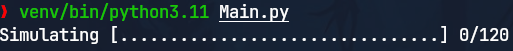
\includegraphics[width=0.7\textwidth]{fig/progressbar.png}
    \caption{Progress bar of the simulations being run in order to get results}\label{fig:progress bar}
\end{figure}

During the execution of the graphical representation, the boats are depicted on
the water at the top of the screen. They appear and disappear as required by
the simulation. The yard is represented by blocks of varying sizes, each
indicating its respective capacity. These blocks are predominantly displayed in
a vibrant green color. It is worth noting that the reefer blocks, which are
used for refrigerated containers, are comparatively smaller in size. The degree
to which a block is filled is represented by the color red. The more red there
is in a block, the more it is filled in terms of percentage.
\begin{figure}
    \centering
    \rotatebox{270}{
        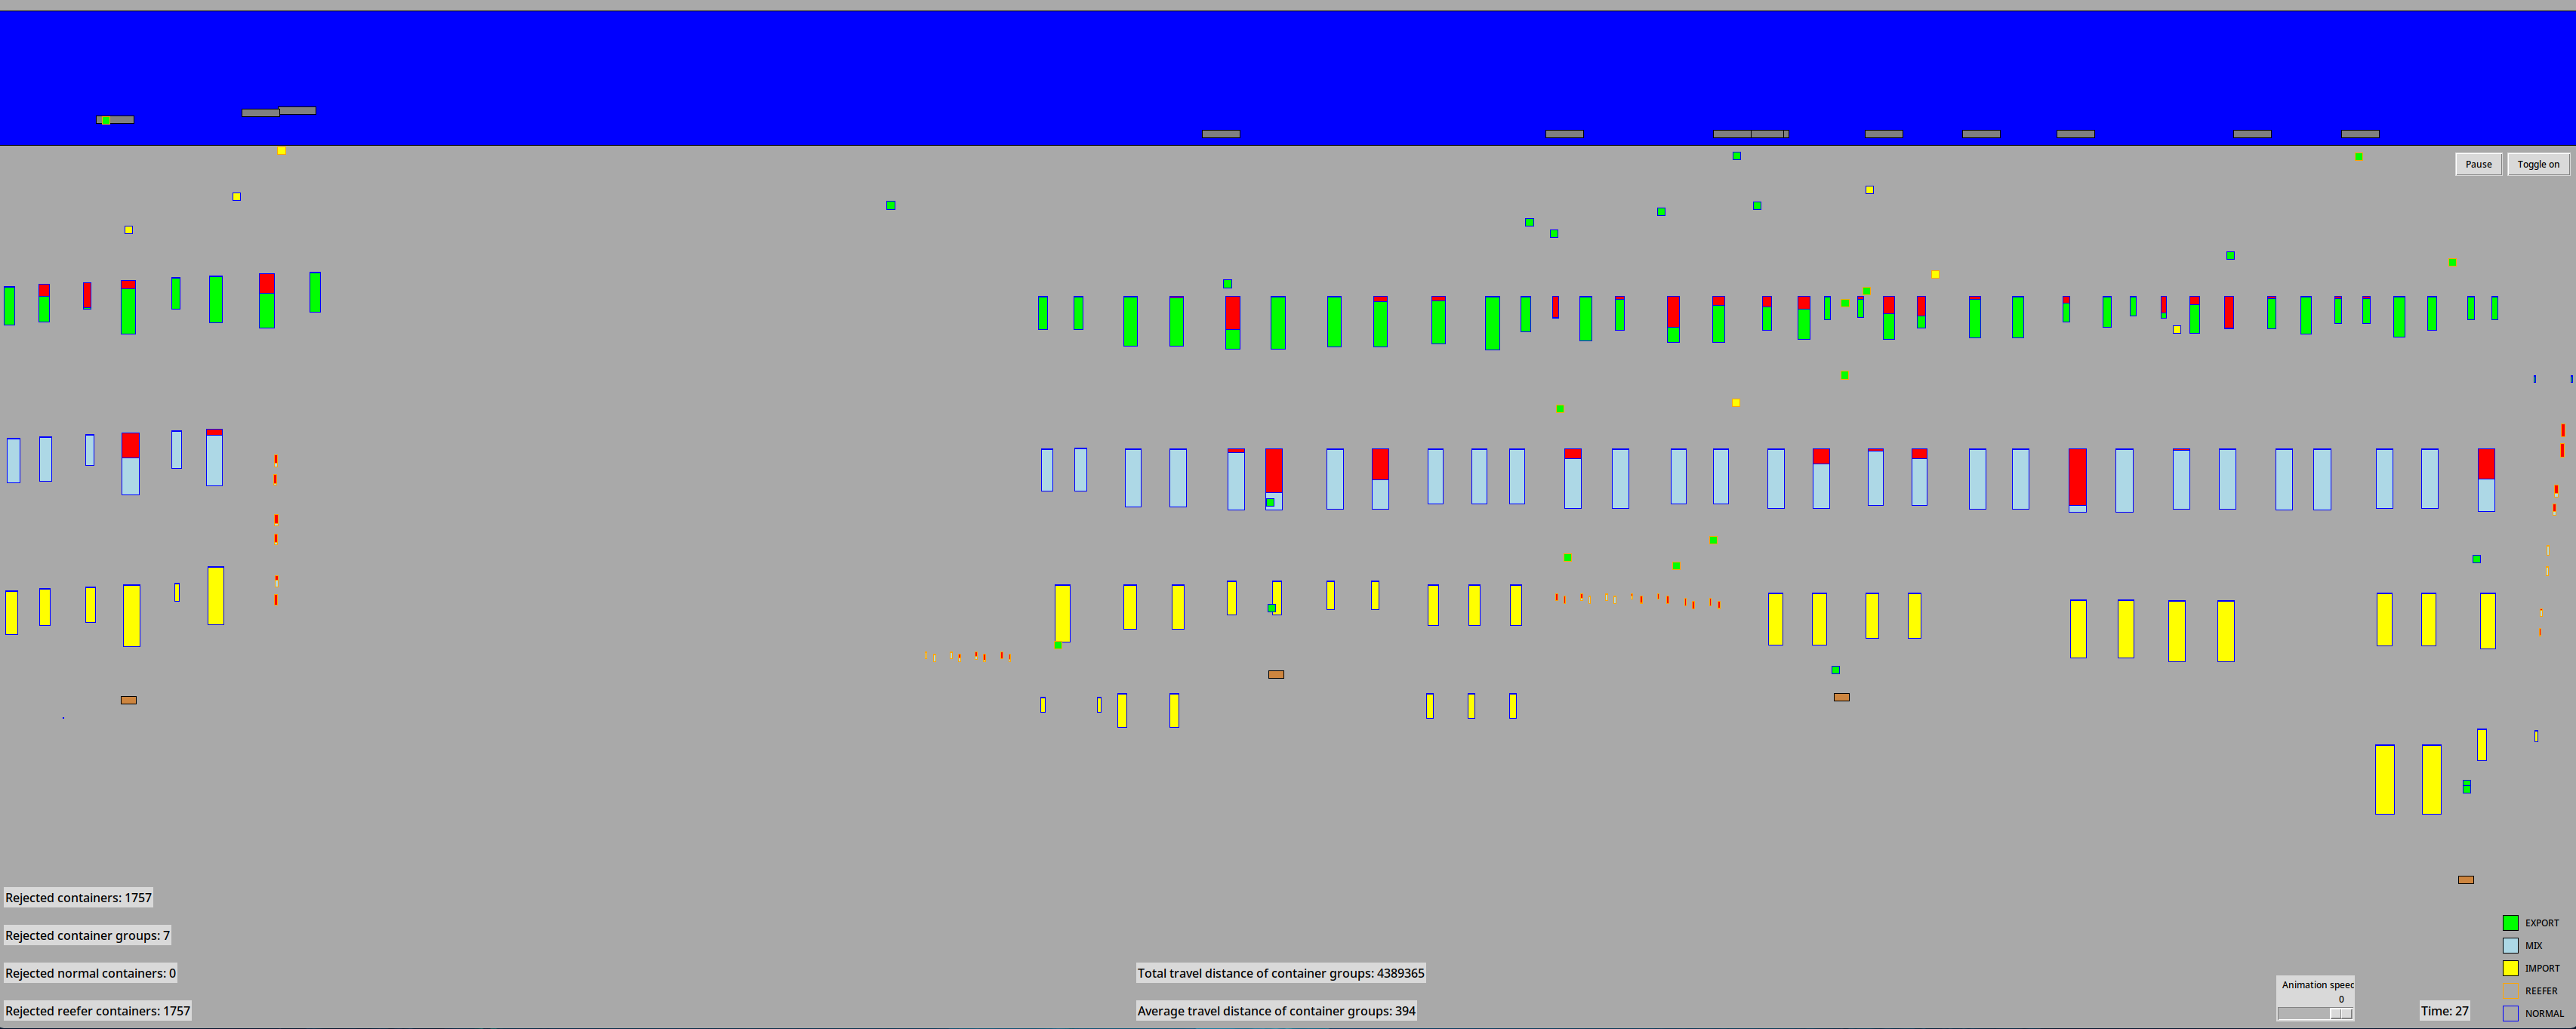
\includegraphics[width=1.4\linewidth]{fig/full GUI.png}
    }
    \caption{Visualization full layout}\label{fig:visualization}
\end{figure}

At the bottom of the screen, various statistics related to the simulation are
displayed, such as the number of rejected containers and the total travel
distance. The legend, indicating the meaning of different colors used in the
visualization, is also located at the bottom for reference.

An interesting feature of the interface is the ability to modify the
simulation's running state on the fly. This means that the simulation can be
paused, allowing for temporary suspension of its progress. Additionally, the
speed of the simulation can be adjusted, allowing users to control the pace of
the simulation. Another option is to toggle the animations on or off. When
animations are turned off, the simulation runs significantly faster, which can
be useful when running the simulation for an extended duration.

\section{What-if scenarios}
A significant aspect of the assignment involved implementing various scenarios
to explore the most "efficient" scenarios or to examine the impact of different
scenarios. This provided an opportunity to test the visualization and gain
insights into the workings of the yard.

As mentioned in previous reports, two different approaches to block assignments
were implemented. These approaches remain applicable to all the scenarios
described in this section. For most scenarios, both approaches to block
assignment are possible. The block assignment rule influences the selection of
a yard block to store a container group. The two situations studied here are
arrival-based and departure-based assignments.

In the case of arrival-based assignment, the chosen yard block is the one
closest to the arrival point. Conversely, in departure-based assignment, the
selected yard block is the one closest to the departure point. In both cases,
the selection is based on minimizing the distance between two points.

\subsection{Base Scenario}
The base scenario remains unchanged from the previous report, where the
decision rule is that a container group is accepted if there is available space
in the yard. This scenario is referred to as FIFO (First In First Out). The
FIFO rule applies to the arrival of containers and determines whether they are
stored in the yard. According to FIFO, the first container group that arrives
is given priority over subsequent arrivals. If there is no space available for
an arriving container group, it will be rejected. The block assignment rule
determines which yard block is assigned to store the respective containers.

We use the base scenario as a reference point for the other scenarios. It is a
scenario where most statistics point to a solid model. Table
\ref{tab:Base_arival} shows the arrival based results. Table
\ref{tab:Base_departure_arrival} shows the arrival and departure based results.
There is a very slight difference in rejected containers between the two
approaches, arrival based has 954 fewer rejected containers. This is a very
small number compared to the total containers rejected. The arrival based
approach has more containergroups rejected compared to arrival and departure
based. The difference in distance travelled between the two approaches is more
significant. The total distance travelled from arrival based is far less than
departure based. The average difference is 168.2 this is a bit less than a 10\%
difference. It is also noticeable that in this scenario that the yard gets
fuller when arrival based is used.

Table \ref{tab:Base_departure} show the departure based results. This approach
has more rejected container groups than the other two approaches. The
difference is still quite slight and probably due to the randomness of the
simulation. However, the difference in travelled distance is more noticeable.
With an increase of 24.5\% compared to arrival based and 13.7\% compared to
arrival and departure based, this could be due to the yard being fuller than
the other two approaches.

\begin{table}[h]
    \centering
    \begin{tabular}{|c|c|}
        \hline
        Containers Rejected                         & 548306.083     \\ \hline
        CG Rejected                                 & 4034.933       \\ \hline
        Normal Rejected                             & 9816.133       \\ \hline
        Reefer Rejected                             & 538489.95      \\ \hline
        Total Travel Distance                       & 5314784151.897 \\ \hline
        AVG Travel Distance Containers              & 1754.928       \\ \hline
        Portion of YB close to full (at some point) & 0.698          \\ \hline
        Portion of YB never used                    & 0.195          \\ \hline
        Portion of YB close to full (average)       & 0.698          \\ \hline
        AVG daily total Occupancy                   & 0.745          \\ \hline
    \end{tabular}
    \caption{Base scenario, distance reference: arrival based}
    \label{tab:Base_arival}
\end{table}
\begin{table}[h]
    \centering
    \begin{tabular}{|c|c|}
        \hline
        Containers Rejected                         & 549260.158    \\ \hline
        CG Rejected                                 & 4029.158      \\ \hline
        Normal Rejected                             & 9932.708      \\ \hline
        Reefer Rejected                             & 539327.45     \\ \hline
        Total Travel Distance                       & 5823736051.32 \\ \hline
        AVG Travel Distance Containers              & 1923.124      \\ \hline
        Portion of YB close to full (at some point) & 0.591         \\ \hline
        Portion of YB never used                    & 0.258         \\ \hline
        Portion of YB close to full (average)       & 0.591         \\ \hline
        AVG daily total Occupancy                   & 0.673         \\ \hline
    \end{tabular}
    \caption{Base scenario, distance: arrival \& departure based}
    \label{tab:Base_departure_arrival}
\end{table}
\begin{table}[h]
    \centering
    \begin{tabular}{|c|c|}
        \hline
        Containers Rejected                         & 551553.892     \\ \hline
        CG Rejected                                 & 4053.15        \\ \hline
        Normal Rejected                             & 12869.05       \\ \hline
        Reefer Rejected                             & 538684.842     \\ \hline
        Total Travel Distance                       & 6622102730.796 \\ \hline
        AVG Travel Distance Containers              & 2184.101       \\ \hline
        Portion of YB close to full (at some point) & 0.648          \\ \hline
        Portion of YB never used                    & 0.05           \\ \hline
        Portion of YB close to full (average)       & 0.648          \\ \hline
        AVG daily total Occupancy                   & 0.842          \\ \hline
    \end{tabular}
    \caption{Base scenario, distance reference: departure based}
    \label{tab:Base_departure}
\end{table}

\subsection{Smallest Remaining capacity}
The first new scenario involves storing all containers of the same container
group in the same yard block. The containers are placed in the yard block with
the largest remaining capacity. This approach ensures that the yard gradually
fills up in a balanced manner across all available storage blocks. However,
there were two possible interpretations for the concept of "remaining capacity"
without explicit emphasis. In this implementation, the choice was made to
consider the absolute number of available container slots in each yard block.
An alternative interpretation could have been to use normalized remaining
capacity, which represents the percentage of capacity that is still available
in each block. In cases where two yard blocks have exactly the same remaining
capacity, the closest one is chosen based on the block assignment rule.

We will compare the results of this scenario to the FIFO scenario. Here we see
that the rejected containergroups is far more than the previous scenario. In
this scenario, the large yard blocks fill up first. This means that the larger
containergroups have no free spot in the yard, which results into rejection.
The distance travelled is also higher than the base scenario. In this scenario,
the distance isn't used in the discussion process to determine where to store
the container group. It is also noticeable that the yard is less full compared
to the previous scenario.

The difference between arrival, departure and arrival \& departure is small.
This is because the scenario decides the location based on size and not on the
distance. The approaches only make a difference when two yard blocks have the
remaining capacity.
\begin{table}[h]
    \centering
    \begin{tabular}{|c|c|}
        \hline
        Containers Rejected                         & 650443.533     \\ \hline
        CG Rejected                                 & 5013.842       \\ \hline
        Normal Rejected                             & 48756.217      \\ \hline
        Reefer Rejected                             & 601687.317     \\ \hline
        Total Travel Distance                       & 8270153316.425 \\ \hline
        AVG Travel Distance Containers              & 2728.917       \\ \hline
        Portion of YB close to full (at some point) & 0.453          \\ \hline
        Portion of YB never used                    & 0.245          \\ \hline
        Portion of YB close to full (average)       & 0.453          \\ \hline
        AVG daily total Occupancy                   & 0.645          \\ \hline
    \end{tabular}
    \caption{Lowest remaining capacity,  distance reference: arrival \& departure based}
\end{table}

\begin{table}[h]
    \centering
    \begin{tabular}{|c|c|}
        \hline
        Containers Rejected                         & 651509.433     \\ \hline
        CG Rejected                                 & 5014.367       \\ \hline
        Normal Rejected                             & 49211.8        \\ \hline
        Reefer Rejected                             & 602297.633     \\ \hline
        Total Travel Distance                       & 8268808654.143 \\ \hline
        AVG Travel Distance Containers              & 2725.312       \\ \hline
        Portion of YB close to full (at some point) & 0.447          \\ \hline
        Portion of YB never used                    & 0.245          \\ \hline
        Portion of YB close to full (average)       & 0.447          \\ \hline
        AVG daily total Occupancy                   & 0.646          \\ \hline
    \end{tabular}
    \caption{Lowest remaining capacity, distance reference: departure based}
\end{table}

\begin{table}[h]
    \centering
    \begin{tabular}{|c|c|}
        \hline
        Containers Rejected                         & 650775.533     \\ \hline
        CG Rejected                                 & 5008.1         \\ \hline
        Normal Rejected                             & 48856.217      \\ \hline
        Reefer Rejected                             & 601919.317     \\ \hline
        Total Travel Distance                       & 8263128846.329 \\ \hline
        AVG Travel Distance Containers              & 2725.798       \\ \hline
        Portion of YB close to full (at some point) & 0.465          \\ \hline
        Portion of YB never used                    & 0.245          \\ \hline
        Portion of YB close to full (average)       & 0.465          \\ \hline
        AVG daily total Occupancy                   & 0.647          \\ \hline
    \end{tabular}
    \caption{Lowest remaining capacity, distance reference: arrival-based}
\end{table}

\subsection{Possible split ups}

In this scenario, container groups have the possibility of being split up into
individual containers, which can be treated separately. This means that a yard
block does not necessarily have to accommodate a full container group.
Consequently, larger container groups should be handled more easily, and
smaller yard blocks can be utilized more effectively within the overall system.

The yard blocks selected to store containers are determined based on their
proximity to the arrival or departure point (depending on the decision rule)
and their available space to accommodate one or more containers. The primary
focus is on identifying the closest block that can hold one or more containers.

BESCHRIJVEN RESULTATEN...

\begin{table}[h]
    \centering
    \begin{tabular}{|c|c|}
        \hline
        Containers Rejected                         & 472353.375     \\ \hline
        CG Rejected                                 & 5127.158       \\ \hline
        Normal Rejected                             & 0.0            \\ \hline
        Reefer Rejected                             & 472353.375     \\ \hline
        Total Travel Distance                       & 5611085409.514 \\ \hline
        AVG Travel Distance Containers              & 1851.933       \\ \hline
        Portion of YB close to full (at some point) & 0.623          \\ \hline
        Portion of YB never used                    & 0.22           \\ \hline
        Portion of YB close to full (average)       & 0.623          \\ \hline
        AVG daily total Occupancy                   & 0.699          \\ \hline
        Average amount of split ups                 & 53848.1        \\ \hline
    \end{tabular}
    \caption{Possible split up, distance: arrival-based}
\end{table}

\begin{table}[h]
    \centering
    \begin{tabular}{|c|c|}
        \hline
        Containers Rejected                         & 473158.492     \\ \hline
        CG Rejected                                 & 5131.692       \\ \hline
        Normal Rejected                             & 0.0            \\ \hline
        Reefer Rejected                             & 473158.492     \\ \hline
        Total Travel Distance                       & 6959654819.095 \\ \hline
        AVG Travel Distance Containers              & 2297.05        \\ \hline
        Portion of YB close to full (at some point) & 0.629          \\ \hline
        Portion of YB never used                    & 0.101          \\ \hline
        Portion of YB close to full (average)       & 0.629          \\ \hline
        AVG daily total Occupancy                   & 0.788          \\ \hline
        Average amount of split ups                 & 65446.74       \\ \hline
    \end{tabular}
    \caption{Possible split up, distance reference: departure based}
\end{table}

\begin{table}[h]
    \centering
    \begin{tabular}{|c|c|}
        \hline
        Containers Rejected                         & 472326.425     \\ \hline
        CG Rejected                                 & 5144.042       \\ \hline
        Normal Rejected                             & 0.0            \\ \hline
        Reefer Rejected                             & 472326.425     \\ \hline
        Total Travel Distance                       & 6077806085.211 \\ \hline
        AVG Travel Distance Containers              & 2006.154       \\ \hline
        Portion of YB close to full (at some point) & 0.547          \\ \hline
        Portion of YB never used                    & 0.321          \\ \hline
        Portion of YB close to full (average)       & 0.547          \\ \hline
        AVG daily total Occupancy                   & 0.613          \\ \hline
        Average amount of split ups                 & 74397.59       \\ \hline
    \end{tabular}
    \caption{Possible split up, distance reference: arrival \& departure based}
\end{table}

\subsection{Not allowing mixing container types in a single yardblock}
The final scenario introduces a rule where MIX yard blocks can only accommodate
containers of a single flow type. This means that once a container arrives and
occupies a MIX yard block, only containers of the same flow type can be added
to that particular yard block. In other words, containers with different flow
types cannot be mixed within the same yard block. This rule ensures segregation
and grouping of containers based on their flow type in the yard.

BESCHRIJVEN RESULTATEN...

\begin{table}[h]
    \centering
    \begin{tabular}{|c|c|}
        \hline
        Containers Rejected                         & 562005.908     \\ \hline
        CG Rejected                                 & 4285.208       \\ \hline
        Normal Rejected                             & 10305.508      \\ \hline
        Reefer Rejected                             & 551700.4       \\ \hline
        Total Travel Distance                       & 5329012083.215 \\ \hline
        AVG Travel Distance Containers              & 1757.727       \\ \hline
        Portion of YB close to full (at some point) & 0.679          \\ \hline
        Portion of YB never used                    & 0.176          \\ \hline
        Portion of YB close to full (average)       & 0.679          \\ \hline
        AVG daily total Occupancy                   & 0.748          \\ \hline
    \end{tabular}
    \caption{Mixed rule, distance reference: arrival-based}
\end{table}

\begin{table}[h]
    \centering
    \begin{tabular}{|c|c|}
        \hline
        Containers Rejected                         & 562459.5       \\ \hline
        CG Rejected                                 & 4311.817       \\ \hline
        Normal Rejected                             & 12785.225      \\ \hline
        Reefer Rejected                             & 549674.275     \\ \hline
        Total Travel Distance                       & 6606445719.566 \\ \hline
        AVG Travel Distance Containers              & 2180.617       \\ \hline
        Portion of YB close to full (at some point) & 0.648          \\ \hline
        Portion of YB never used                    & 0.044          \\ \hline
        Portion of YB close to full (average)       & 0.648          \\ \hline
        AVG daily total Occupancy                   & 0.842          \\ \hline
    \end{tabular}
    \caption{Mixed rule, distance reference: departure based}
\end{table}

\begin{table}[h]
    \centering
    \begin{tabular}{|c|c|}
        \hline
        Containers Rejected                         & 557756.75     \\ \hline
        CG Rejected                                 & 4226.058      \\ \hline
        Normal Rejected                             & 9384.333      \\ \hline
        Reefer Rejected                             & 548372.417    \\ \hline
        Total Travel Distance                       & 5823224027.74 \\ \hline
        AVG Travel Distance Containers              & 1922.426      \\ \hline
        Portion of YB close to full (at some point) & 0.61          \\ \hline
        Portion of YB never used                    & 0.245         \\ \hline
        Portion of YB close to full (average)       & 0.61          \\ \hline
        AVG daily total Occupancy                   & 0.678         \\ \hline
    \end{tabular}
    \caption{Mixed rule, distance reference: arrival \& departure based}
\end{table}

\section{Performance}\label{sec:performance}

The entire simulation was implemented in Python, which is an interpreted
programming language. Unlike compiled languages like C or C++, Python is
executed by an interpreter rather than being compiled into machine code. As a
result, Python can be perceived as slower in terms of performance compared to
compiled languages.

The simulations were conducted over a period of one year, which involved
extensive computations. When running the simulations without animations, the
average time per simulation was 127.24 seconds. While this may not seem
excessively high, considering the number of simulations required to obtain
meaningful results, it becomes a significant factor. For instance, running 100
simulations would take approximately 3 hours and 32 minutes.

The graphical aspect of the simulation is fully multithreaded, with each moving
container assigned its own thread. This enables smooth animations and enhances
the visual experience. However, this also poses challenges when attempting to
run the simulation multiple times while simultaneously displaying the
visualization, particularly on less powerful computers. Performing such tasks
on separate threads becomes complex due to the already resource-intensive
nature of the visualization process.

\section{Conclusion}
\end{document}